\RequirePackage{luatex85}
\documentclass[tikz]{standalone}
\usepackage{amsmath}
\begin{document}
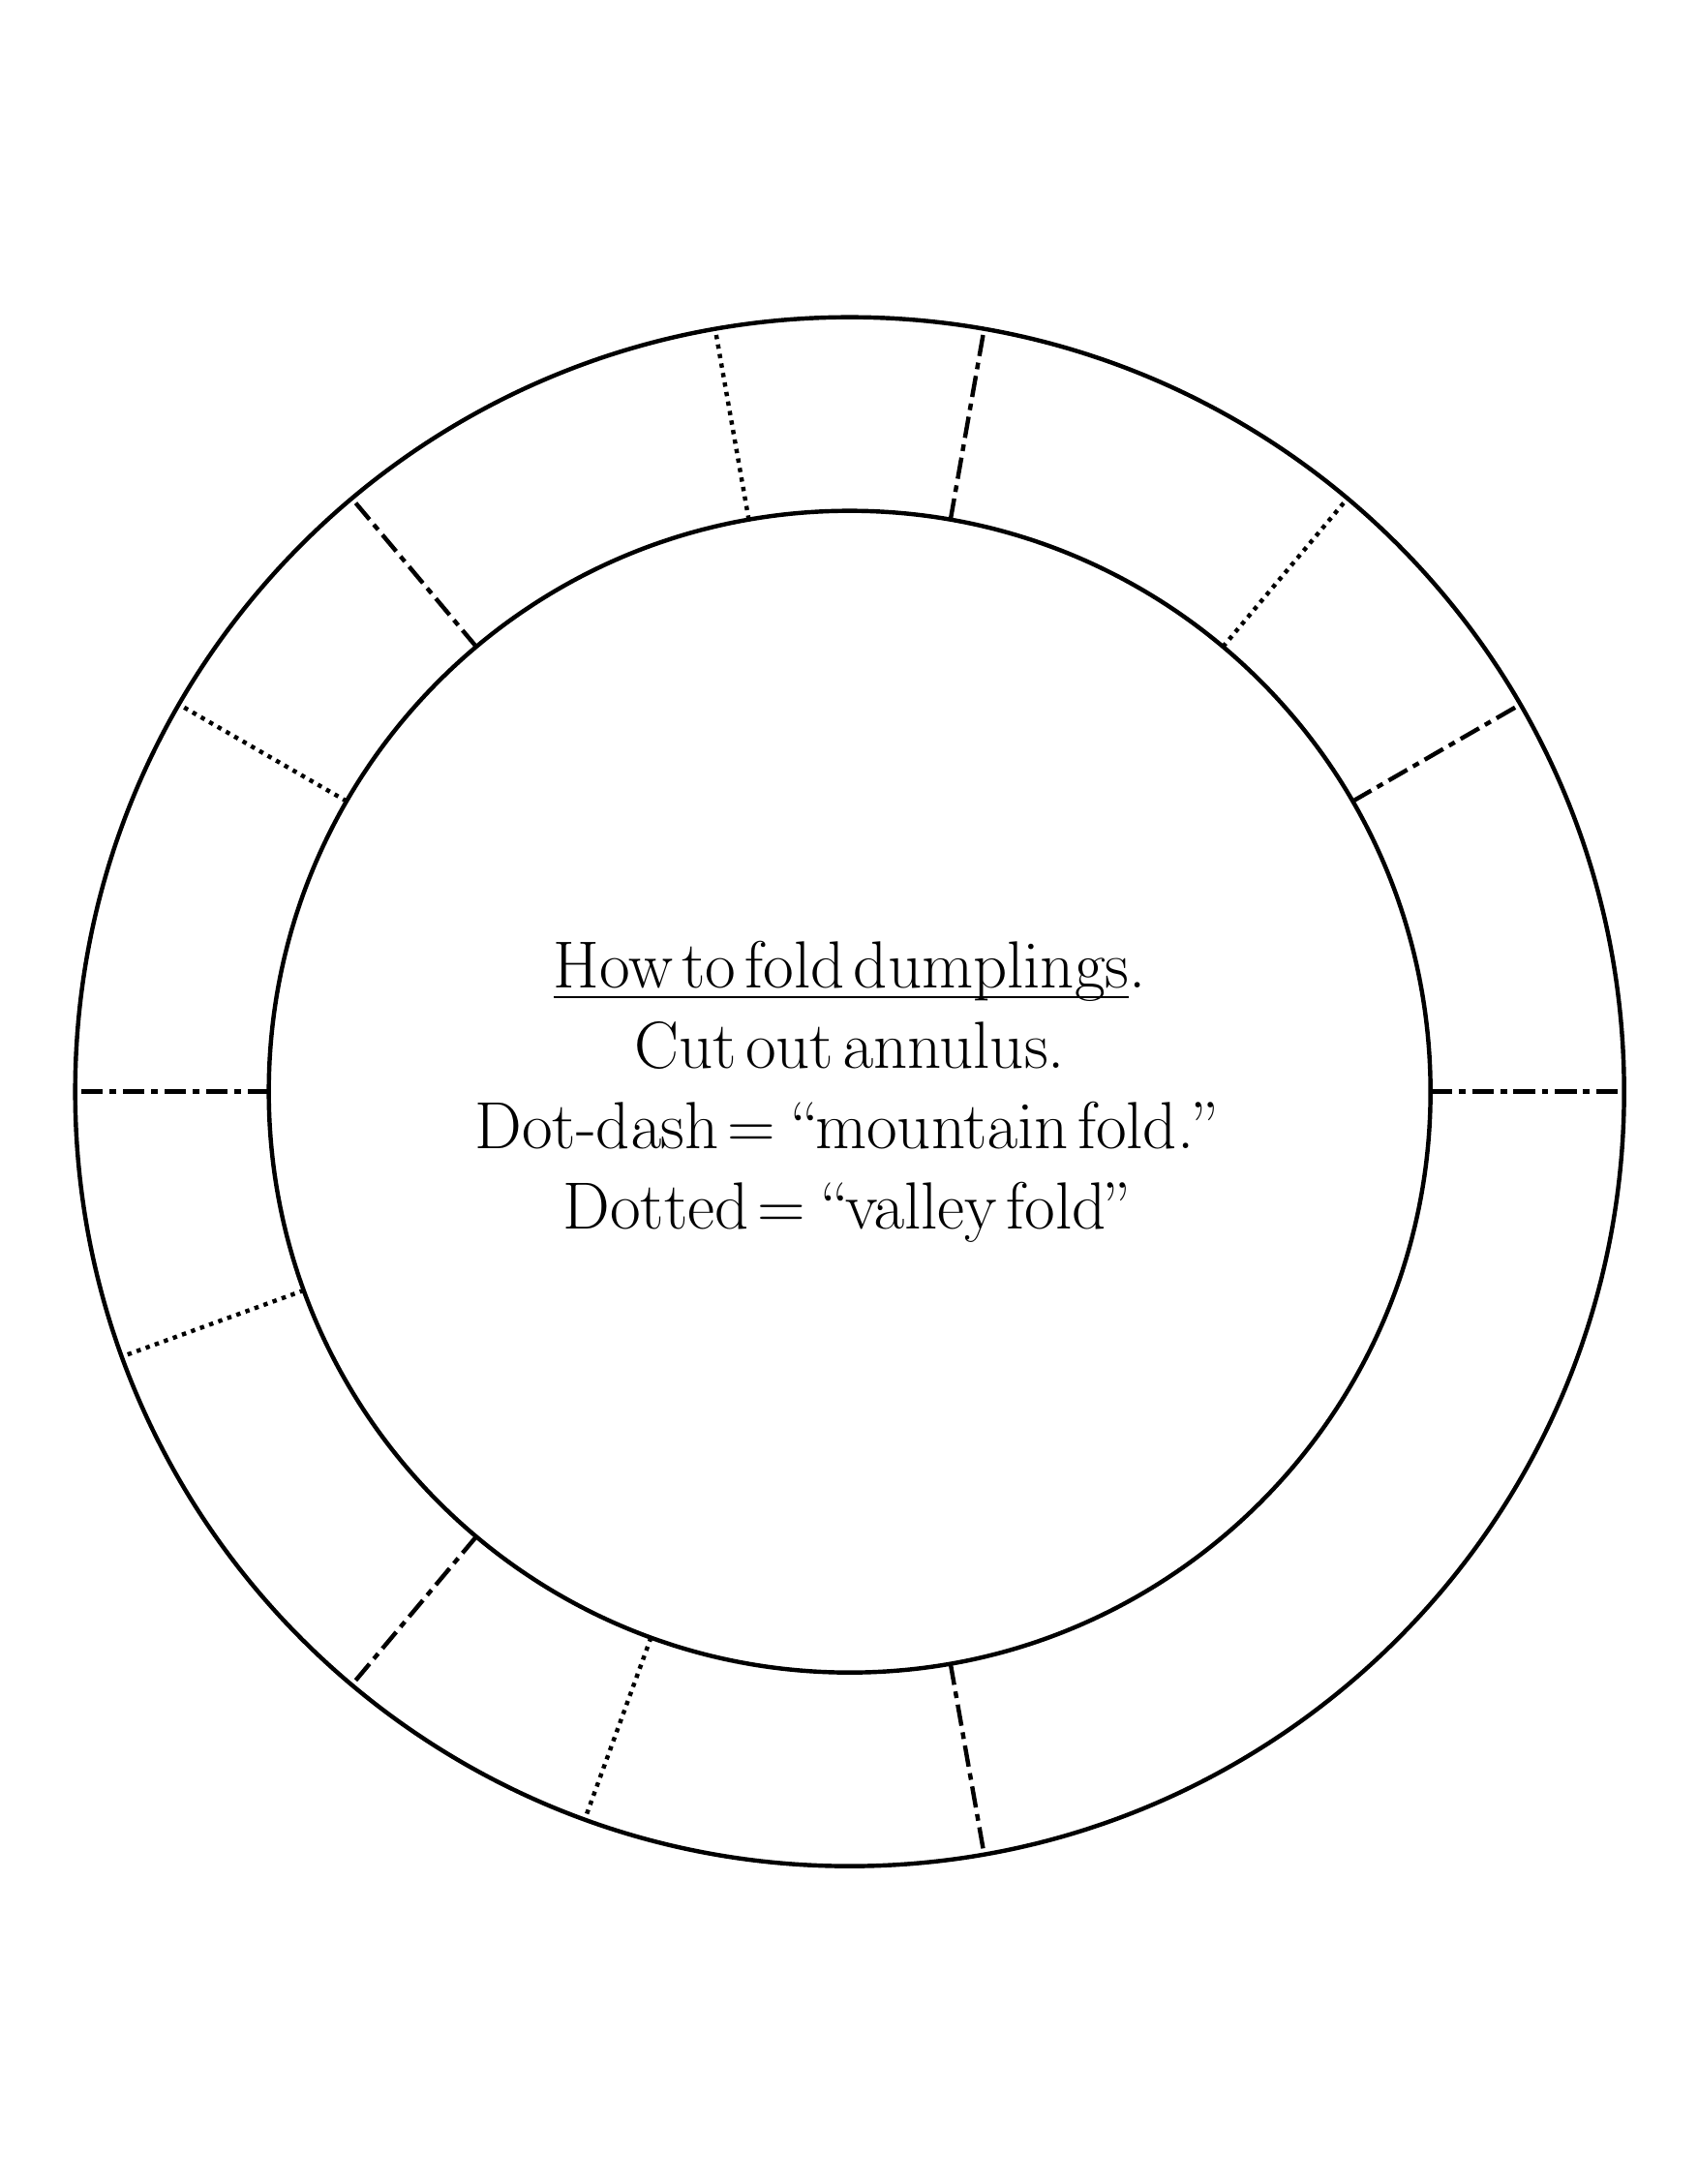
\begin{tikzpicture}[ultra thick]
\clip (-4.25in, -5.5in) rectangle (4.24in, 5.5in);
\draw (0,0) circle (3in);
\draw (0,0) circle (4in);
\foreach \theta in {0, 30, 80, ..., 280}
\draw[dash pattern={on 8pt off 2.5pt on 2.5pt off 2.5pt}]
	(0,0) ++(\theta:3in) -- ++(\theta:1in);
\foreach \theta in {50, 100, ..., 250}
\draw[dotted]
	(0,0) ++(\theta:3in) -- ++(\theta:1in);
\node[text width=4in] (0,0) {\centering\Huge
	\underline{How to fold dum\smash plin\smash gs}. \\
	Cut out annulus. \\ 
	Dot-dash = ``mountain fold." \\
	Dotted = ``valley fold" \\
	};
\end{tikzpicture}
\end{document}